\documentclass[10pt]{beamer}

\usetheme{metropolis}
\usepackage{appendixnumberbeamer}

\usepackage{booktabs}
\usepackage[scale=2]{ccicons}

\usepackage{pgfplots}
\usepgfplotslibrary{dateplot}

\usepackage{xspace}
\newcommand{\themename}{\textbf{\textsc{metropolis}}\xspace}


\usepackage{xcolor}
\usepackage{listings}
\usepackage{caption}
\DeclareCaptionFont{white}{\color{white}}
\DeclareCaptionFormat{listing}{%
	\parbox{\textwidth}{\colorbox{gray}{\parbox{\textwidth}{#1#2#3}}\vskip-4pt}}
\captionsetup[lstlisting]{format=listing,labelfont=white,textfont=white}
\lstset{frame=lrb,xleftmargin=\fboxsep,xrightmargin=-\fboxsep}

\lstset{
	% numbers=left,
	breaklines=true,
	% backgroundcolor=\color{light-gray},
	tabsize=4,
	% basicstyle=\ttfamily,
	literate={\ \ }{{\ }}1	
}


\title{Master Thesis Proposal}
\subtitle{Compliant Manipulation with Reinforcement Learning Guided by Task Specification}
\date{\today}
\author{Abhishek Padalkar}
\institute{Hochschule Bonn-Rhein-Sieg, Sankt Augustin}
% \titlegraphic{\hfill
\includegraphics[height=1.5cm]{logo.pdf}}

\begin{document}

\maketitle

\begin{frame}{Table of contents}
  \setbeamertemplate{section in toc}[sections numbered]
  \tableofcontents[hideallsubsections]
\end{frame}

\section{Introduction}

\begin{frame}[fragile]{Compliant Manipulation}
	\begin{itemize}
		\item Most of the real world robotic manipulation tasks present the need for compliant manipulation.
		\item Robot needs to respond to the contact forces while executing the task. 
		\item Classical planning and control algorithm fail to perform satisfactorily due to the lack of precise model of contact forces and high computational complexity.
	\end{itemize}
\end{frame}

\section{Problem Statement}

\begin{frame}{Problem Statement}
	
	\begin{itemize}
		\item We propose to do use reinforcement learning along with task frame formalism in order to reduce the number of interactions with the environment.
		\item We will evaluate our approach based by learning the task of opening door and cutting vegetables.
	\end{itemize}
\end{frame}
\begin{frame}[fragile]{Task Specification by Meson et. al. \cite{mason1981compliance}}
	
	\begin{lstlisting}[label=tff,caption=Task Specification using TFF: Open Door]
		move compliantly {
			with task frame directions
			xt: force 0 N
			yt: force 0 N
			zt: velocity v mm/sec
			axt: force 0 Nmm
			ayt: force 0 Nmm
			azt: force 0 Nmm
		} until distance > d mm 
	\end{lstlisting}
	

\end{frame}


\begin{frame}{Composition}
	\begin{figure}[!h]
		\center{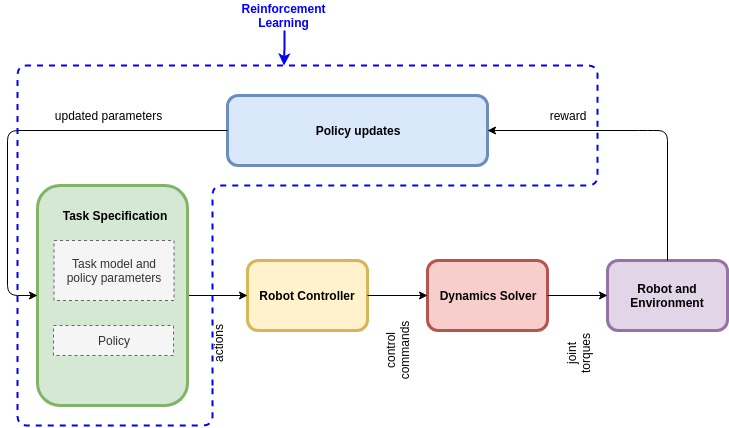
\includegraphics[width=\textwidth]
			{images/composition.png}}
		\caption{\label{fig:composition} Composition}
	\end{figure}
\end{frame}
	


\begin{frame}[allowframebreaks]{References}

  \bibliography{../../project-proposal/bibliography}
  \bibliographystyle{abbrv}

\end{frame}

\end{document}
